\documentclass{beamer}
\usetheme{Darmstadt}
\usecolortheme{beaver}


\usepackage[utf8]{inputenc}
\usepackage{booktabs}
\usepackage{adjustbox}
\usepackage{pbox}

\usepackage[group-separator={\ }, round-mode = places, round-precision = 2]{siunitx}
\usepackage{graphicx}
\DeclareGraphicsExtensions{{.pdf, .png, .jpg}}
\graphicspath{ {images/} }

\usepackage{graphicx}
\usepackage {tikz}
\usetikzlibrary{arrows}
\usetikzlibrary{shapes.misc, positioning, shapes.geometric}
\usepackage{algpseudocode}

\usepackage[backend=biber]{biblatex}
\addbibresource{presentation.bib}
\setbeamertemplate{navigation symbols}{}



\author[]{Reid McIlroy-Young}
\date{March 21, 2019}
\title{Gab, Does it Ever Change?}
\begin{document}

\begin{frame}
\titlepage
\end{frame}

\begin{frame}
\frametitle{Questions}
	\begin{itemize}
	\item Did the site shutdown measurably effect the site's speech?
	\item Are there other underlying trends in the site?
	\item Can we find trends in the hate speech?
\end{itemize}
\end{frame}	

\begin{frame}
\frametitle{Gab}

Snowball sampling of Gab, last run March 27
\begin{table}[h]
	\centering
	\begin{tabular}{lrrr}
		\toprule
		&Before&After&Total\\
		Number Registered Users &712,093&123,602&835,695\\
		Users with Posts& 265,900& 93,684&307,623\\
		Number of Posts& 22,567,328& 9,078,113&31,645,441\\
		Words &&&423,539\\
		\bottomrule
	\end{tabular}
\end{table}
\end{frame}

\begin{frame}
\frametitle{Other Data}

\begin{itemize}
\item Reddit 
\begin{itemize}
	\item All comments made during October 2018
	\item 112,573,001 Posts 
	\item 271,400 words in vocabulary (above 50 occurrences)
\end{itemize}
\item  Google News Word2vec - pretrained
\begin{itemize}
	\item Baseline word2vec for comparisons
	\item 3,000,000 words in vocabulary (case sensitive)
\end{itemize}
\end{itemize}
\end{frame}

\begin{frame}
\frametitle{Gab Usage, Before and After }
\begin{figure}
	\centering
	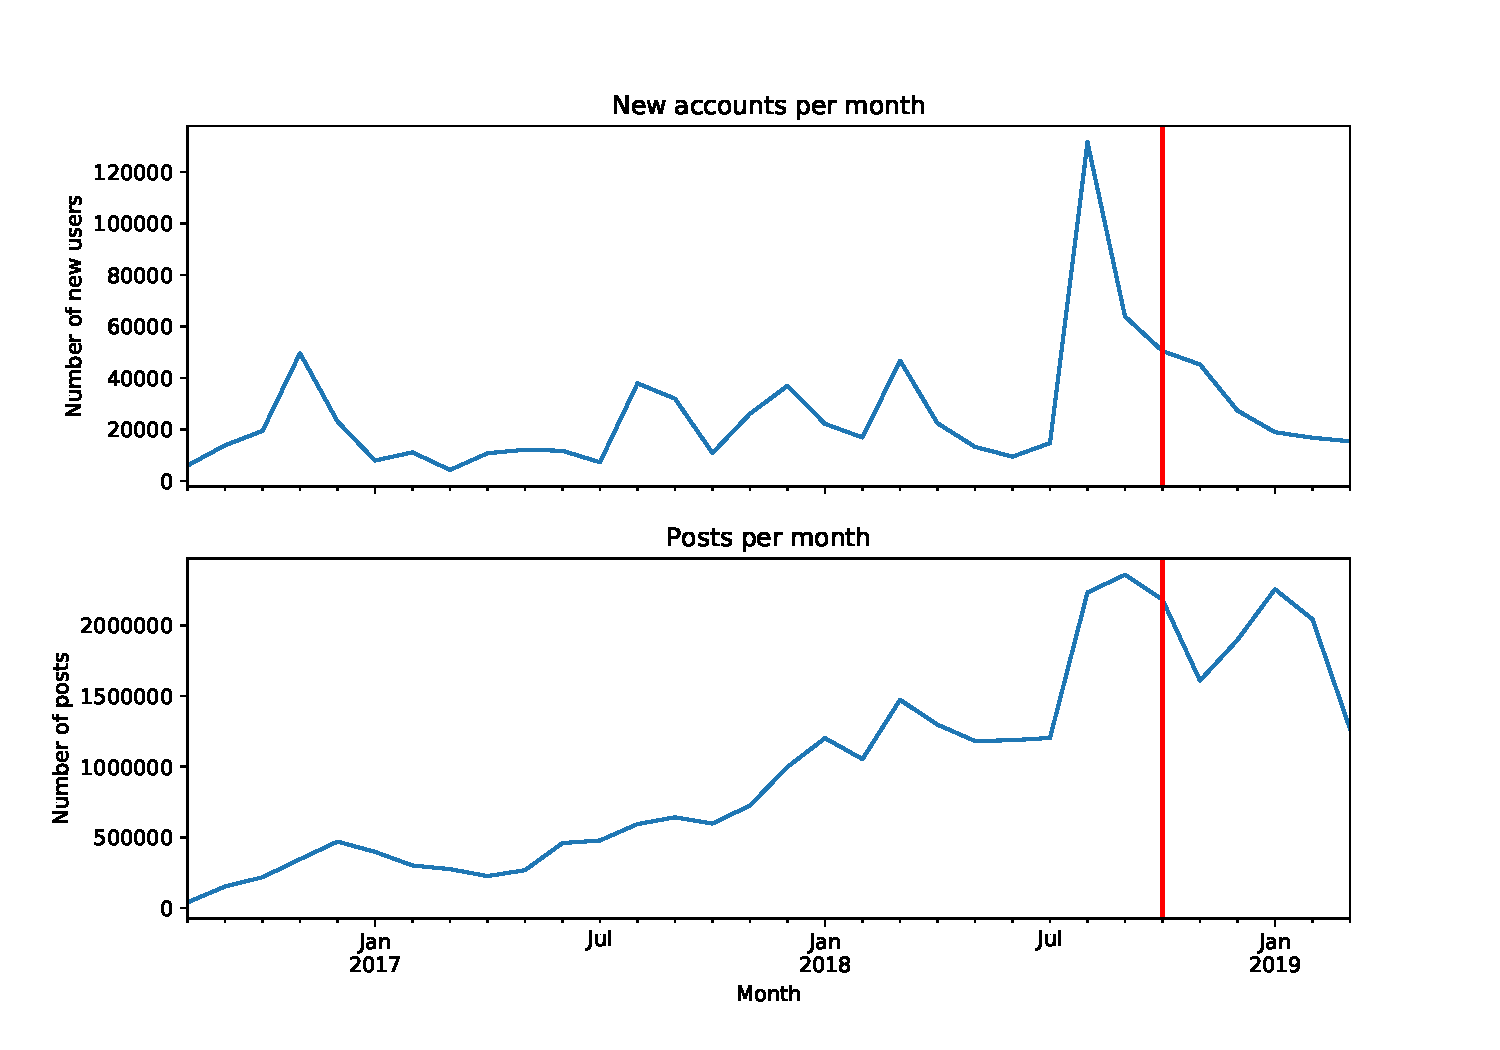
\includegraphics[width=.85\textwidth]{Before_and_after_counts.pdf}
	\caption{Site usage, with the shooting indicated with the red line}
\end{figure}
\end{frame}	

\begin{frame}
\frametitle{Top trigrams from After, by Month}
\begin{figure}
	\centering
	\makebox[0pt]{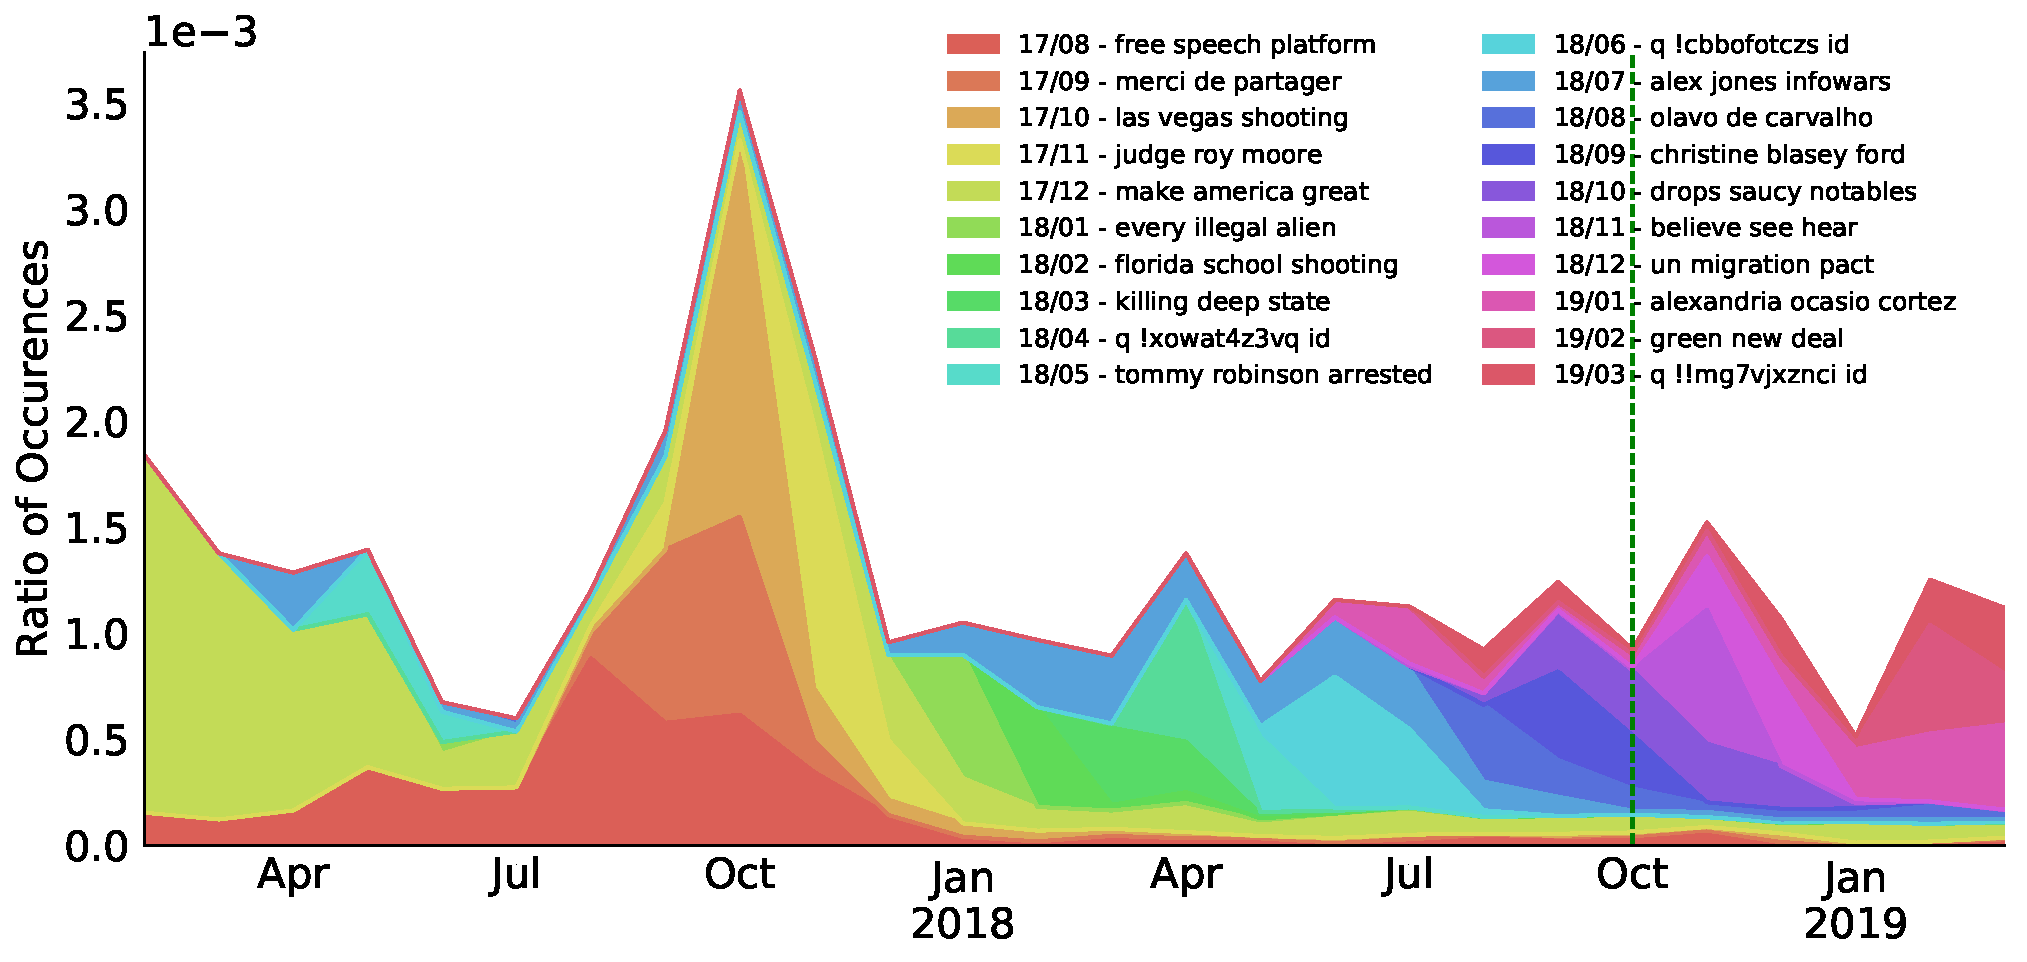
\includegraphics[width=1\textwidth]{trigrams_norepost.pdf}}
	\caption{By month top new trigrams, with the shooting indicated with the line}
\end{figure}
\end{frame}	
\begin{frame}


\frametitle{Anti-Semitic words}
\begin{figure}
\centering
\makebox[0pt]{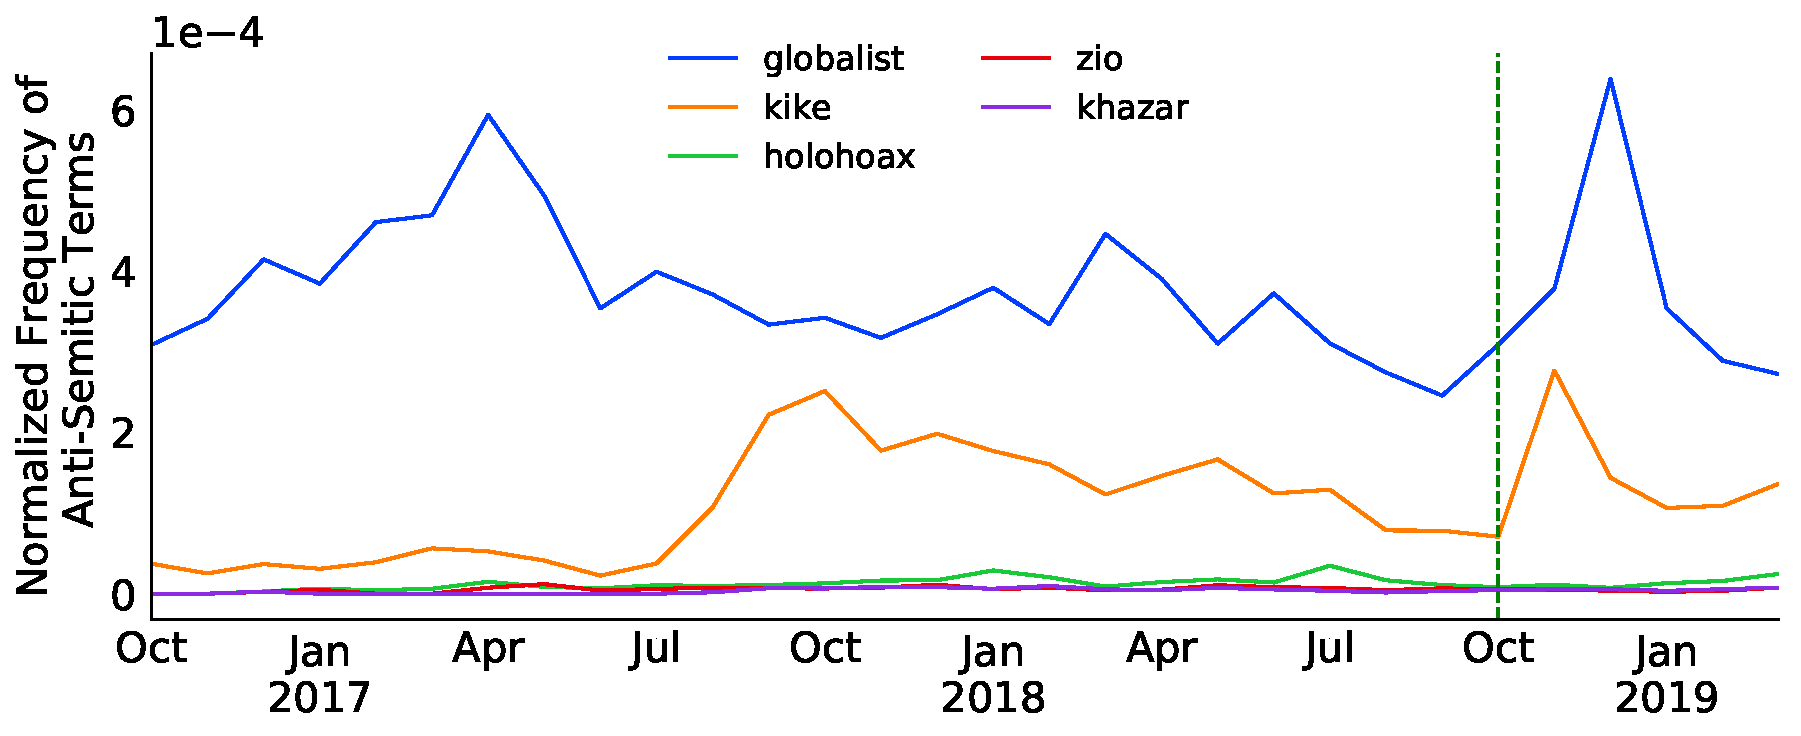
\includegraphics[width=1\textwidth]{overtime_normalized_antisem.pdf}}
\caption{By month ratio of occurrence of the top 5 anti-Semitic words via hatebase.org, with the shooting indicated with the  line}
\end{figure}
\end{frame}	

\begin{frame}
\frametitle{Trained Word2vecs}
\begin{itemize}
	\item[Before] All posts before on Gab the shutdown 
	\item[After] All posts on Gab after the shutdown
	\item[Monthly] Models trained on posts from each month since Gab's creation, 32 in total
	\item[Reddit] All posts on Reddit in October 2018
	\item[Google] The Google news pre trained word2vec
\end{itemize}
The Word2Vecs were all trained with a windows size of 10, and 300 dimensions, and a few  other hyper parameters that were tuned with an analogies task
\end{frame}	

\begin{frame}
\frametitle{Differences between words}
\begin{figure}
	\centering
	\makebox[0pt]{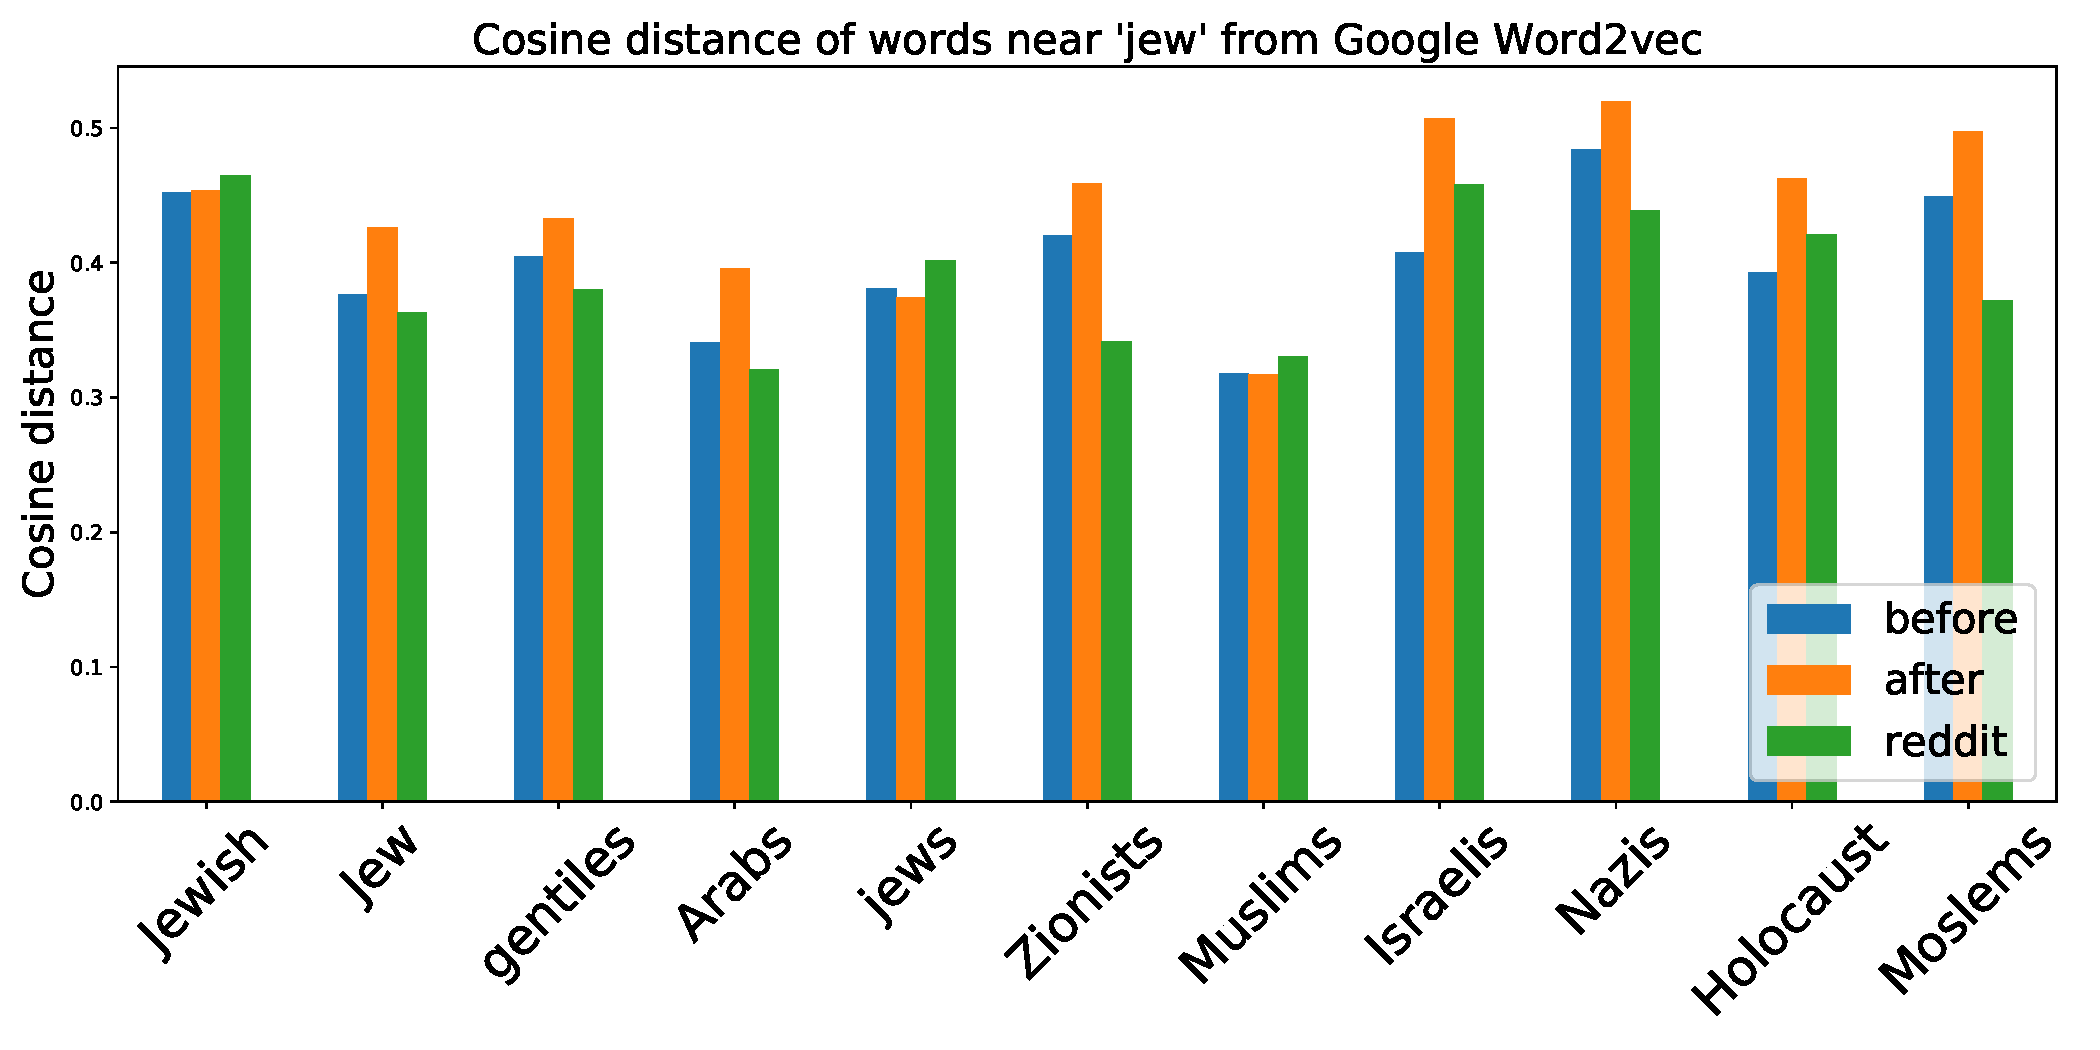
\includegraphics[width=1\textwidth]{sim_bars_jewish.pdf}}
	\caption{Cosine distance of different words from Google to aligned word2vecs}
\end{figure}
\end{frame}	

\begin{frame}
\frametitle{Differences between words}
\begin{figure}
	\centering
	\makebox[0pt]{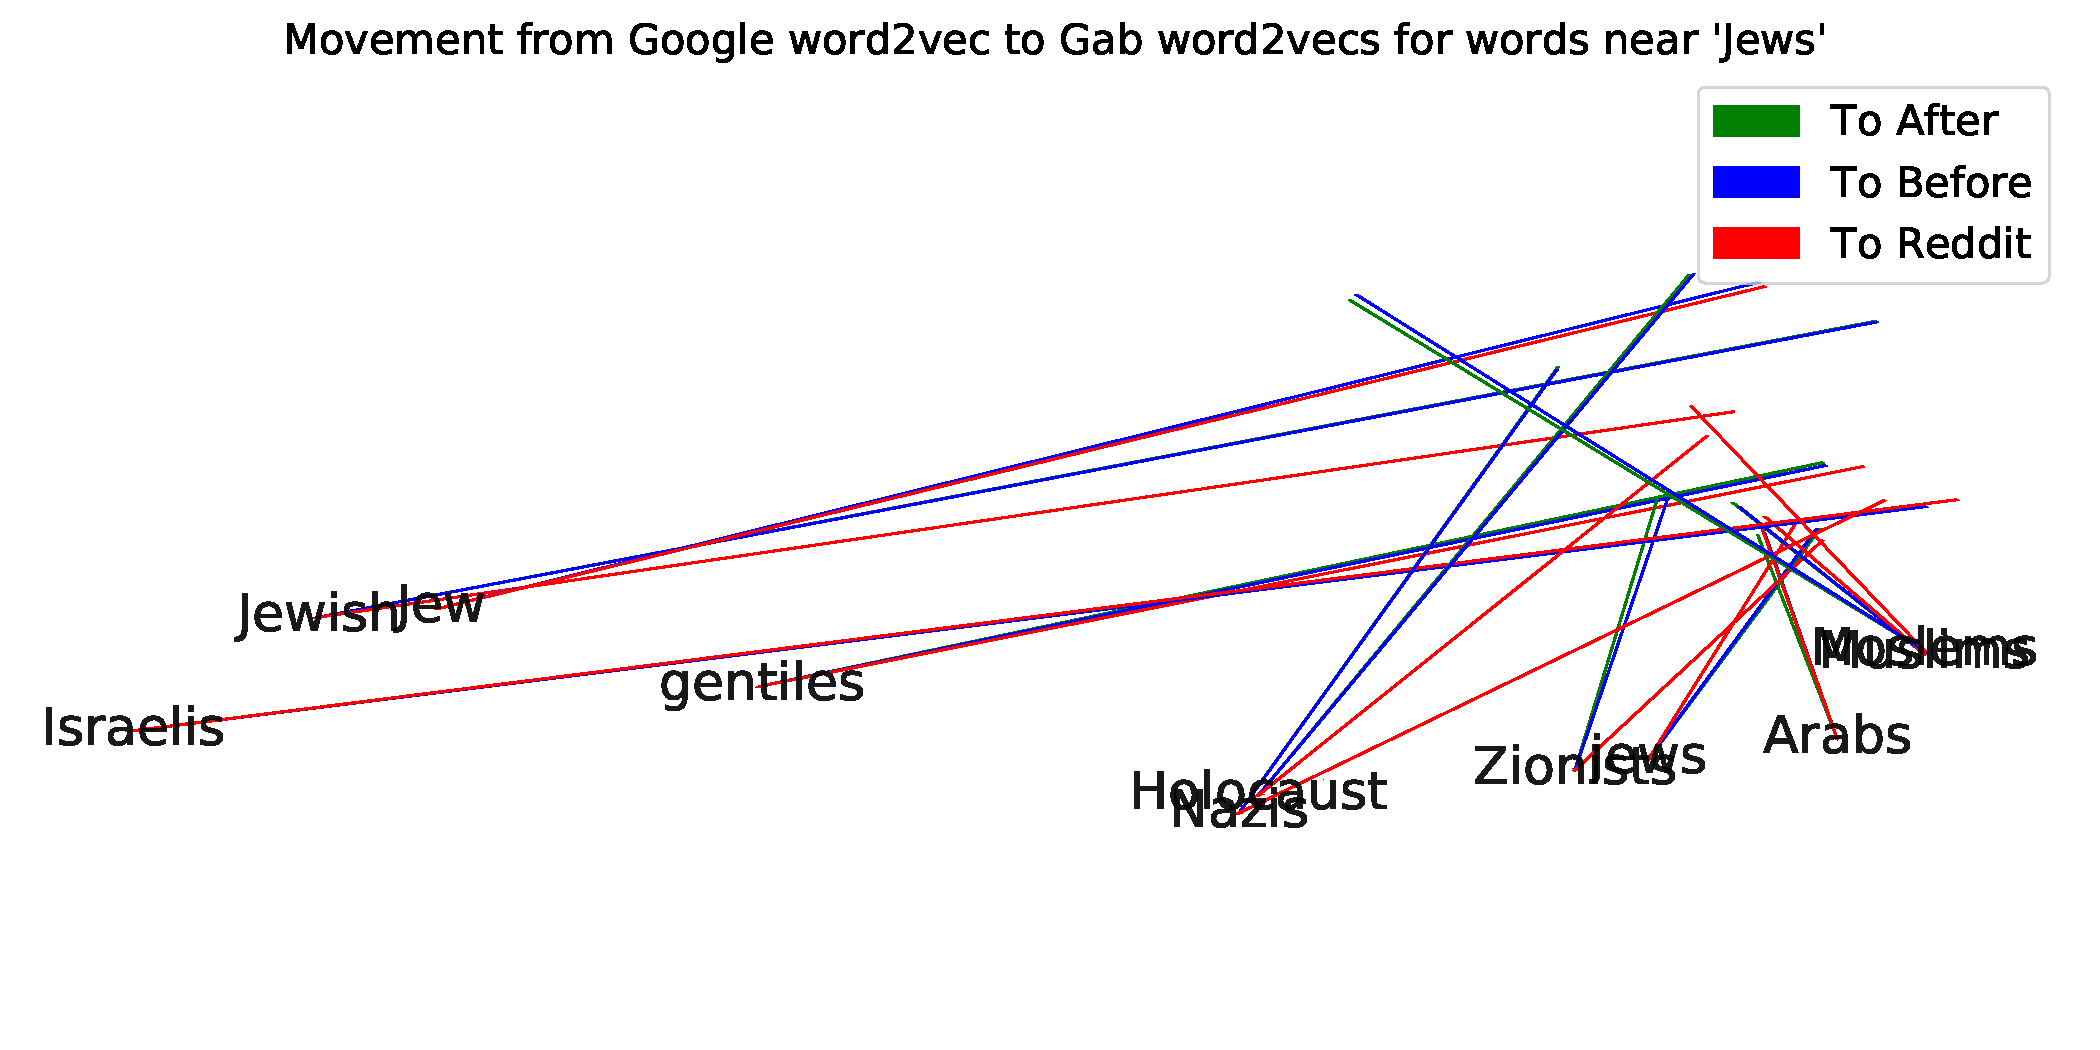
\includegraphics[width=1\textwidth]{tsen_jewish_arrows.pdf}}
	\caption{t-SNE embedding of all 4 aligned word2vecs, lines show movement from Google to to other Word2Vecs}
\end{figure}
\end{frame}	

\begin{frame}
\frametitle{Monthly Cosine Distances}
\begin{figure}
	\centering
	\makebox[0pt]{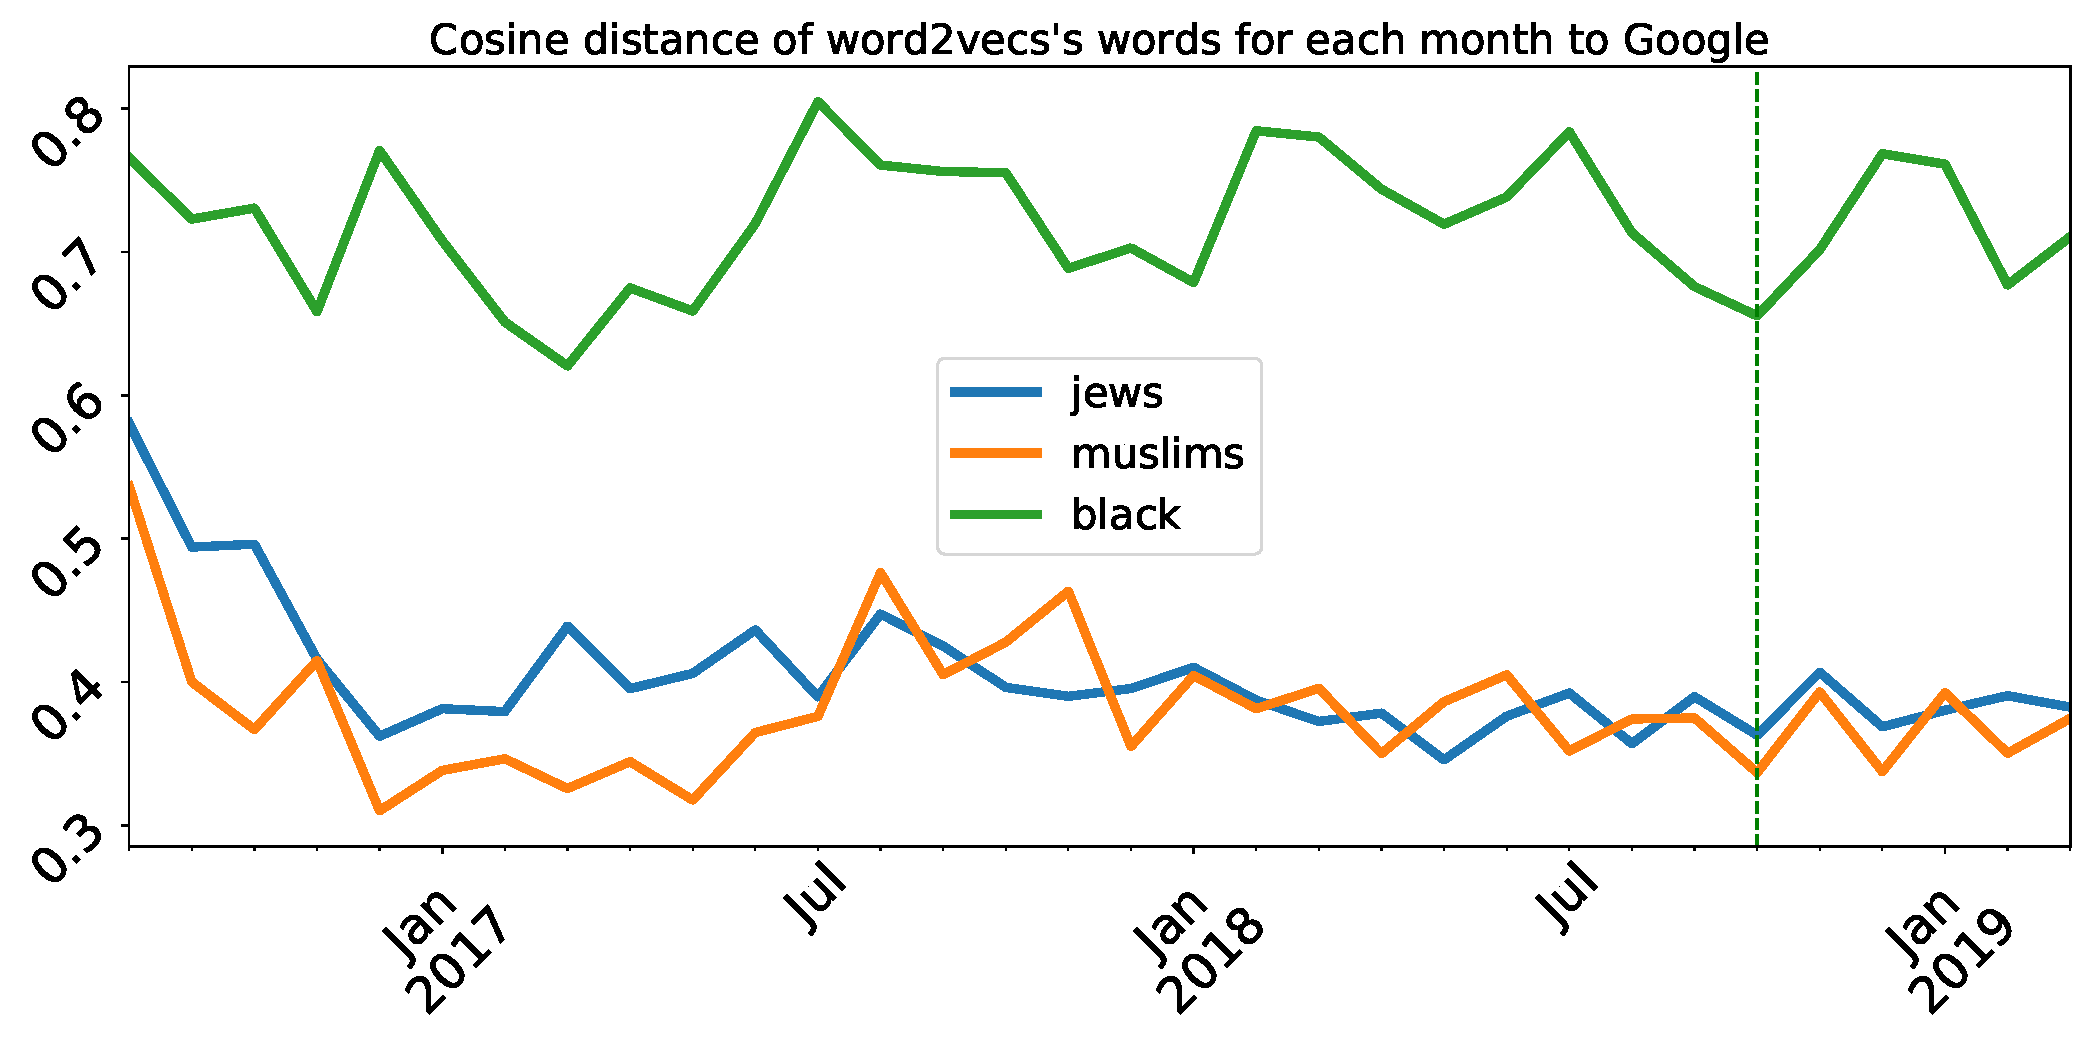
\includegraphics[width=1\textwidth]{sim_ethnic_jewish.pdf}}
	\caption{Distance from Google for select words by month}
\end{figure}
\end{frame}	

\begin{frame}
\frametitle{Monthly Cosine Distances}
\begin{figure}
	\centering
	\makebox[0pt]{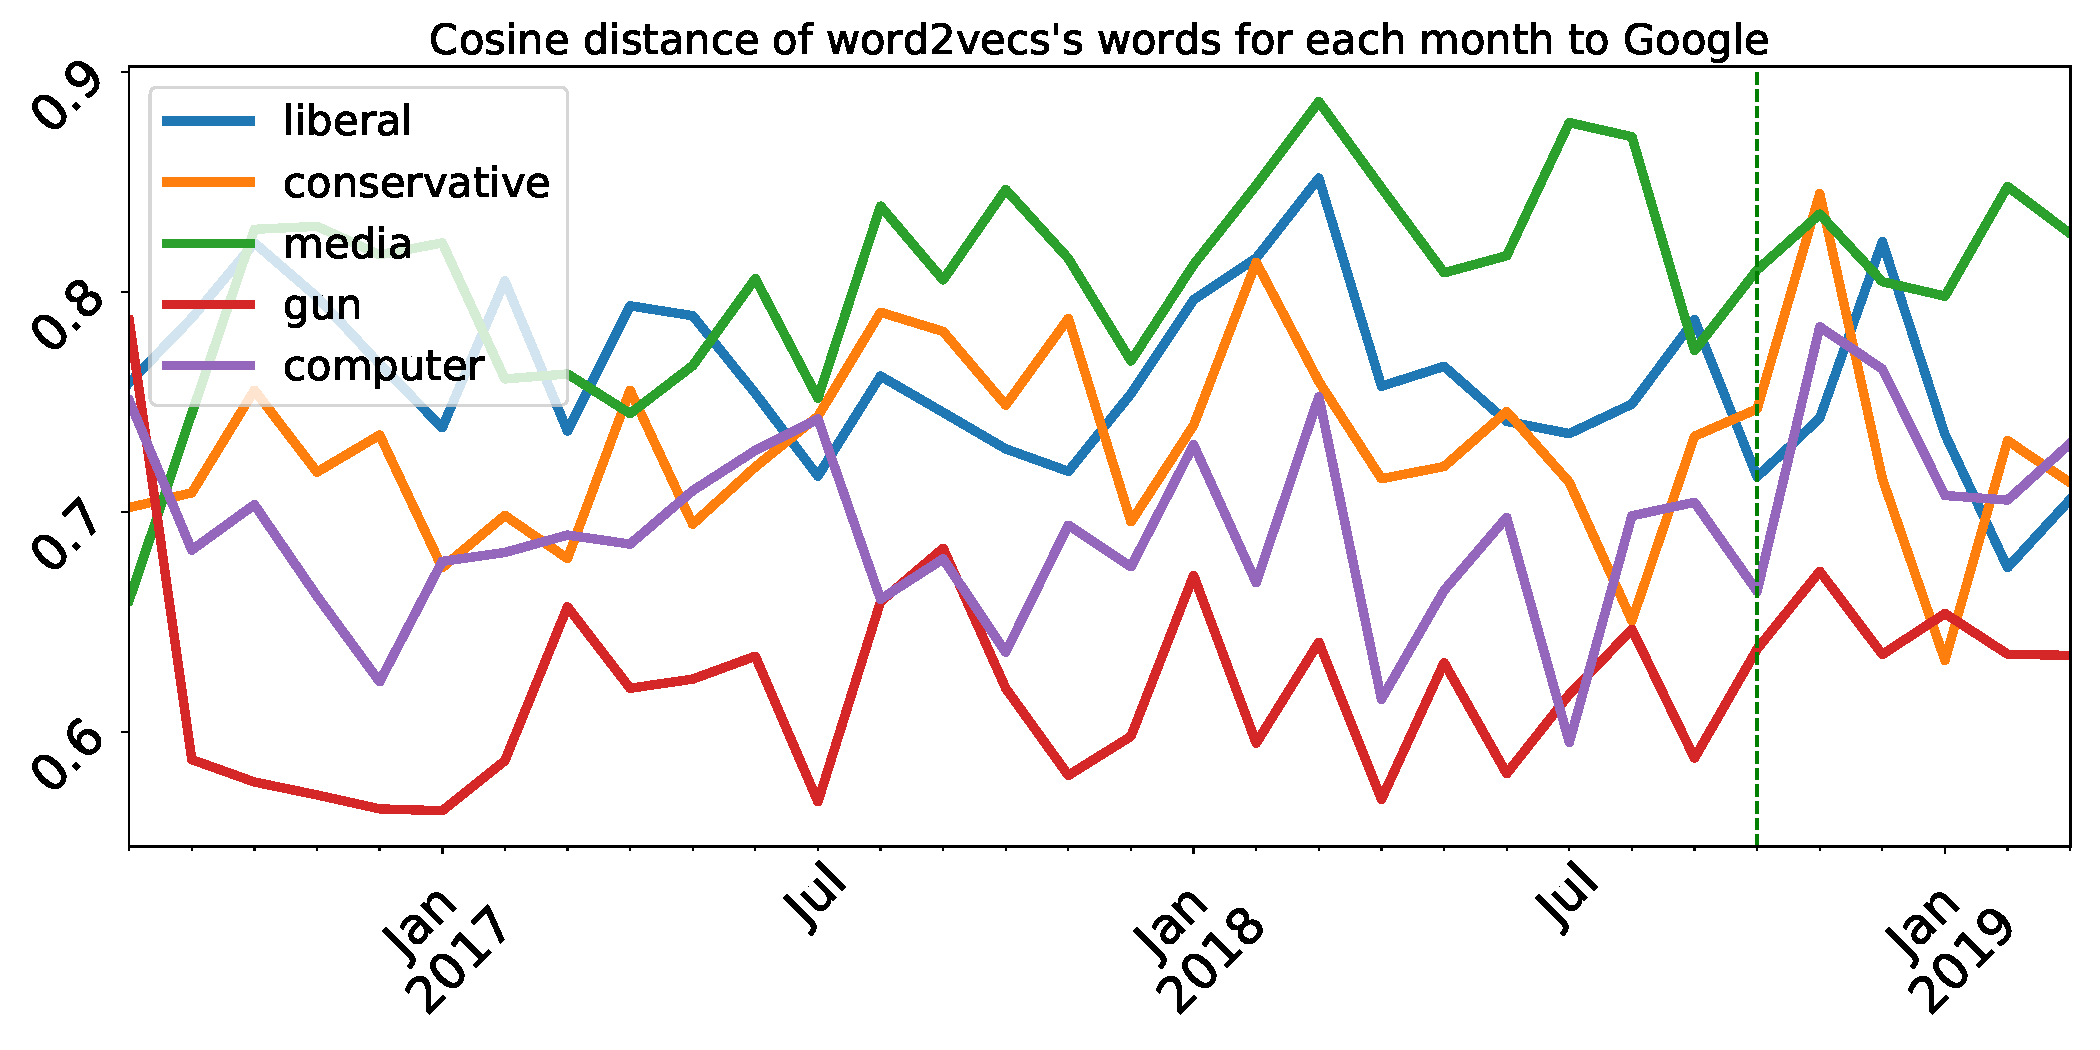
\includegraphics[width=1\textwidth]{sim_misc_jewish.pdf}}
	\caption{Distance from Google for select words by month}
\end{figure}
\end{frame}	

\begin{frame}
\frametitle{Least and Most Likely Words}
	\begin{table}[t]
		\centering
		\small
		\begin{tabular}{lr|lr}
			\toprule
			Word &  Log Odds &  Word  & Log Odds \\
			\midrule
			ballots         &   2.82517  &  gillette        &  -4.32011\\
			dec             &   2.68070  &  bonner          &  -4.12487\\
			broward         &   2.50657  &  christchurch    &  -3.93367\\
			oven            &   2.26191  &  alckmin         &  -3.83449\\
			nov             &   2.21719  &  ford’s          &  -3.64577\\
			compact         &   2.12065  &  candidatos      &  -3.49373\\
			thanksgiving    &   2.07243  &  covington       &  -3.48308\\
			acosta          &   2.01614  &  1d              &  -3.27645\\
			christmas       &   1.97001  &  candidato       &  -3.20228\\
			merry           &   1.85361  &  omarosa         &  -2.63009\\
			december        &   1.77640  &  uol             &  -2.60407\\
			macron          &   1.76386  &  marina          &  -2.59409\\
			\bottomrule
		\end{tabular}
		\caption{Words with the lowest and highest log odds of occurring in After from the top 10,000 words by count in After}
	\end{table}
\end{frame}

\begin{frame}
\frametitle{Questions?}

\end{frame}

\end{document}